\documentclass{article}
\usepackage[margin=1in]{geometry}
\usepackage[linesnumbered,ruled,vlined]{algorithm2e}
\usepackage{amsfonts}
\usepackage{amsmath}
\usepackage{amssymb}
\usepackage{amsthm}
\usepackage{enumitem}
\usepackage{fancyhdr}
\usepackage{hyperref}
\usepackage{minted}
\usepackage{multicol}
\usepackage{pdfpages}
\usepackage{standalone}
\usepackage[many]{tcolorbox}
\usepackage{tikz-cd}
\usepackage{transparent}
\usepackage{xcolor}
% \tcbuselibrary{minted}

\author{Nathan Solomon}

\newcommand{\fig}[1]{
    \begin{center}
        \includegraphics[width=\textwidth]{#1}
    \end{center}
}

% Math commands
\renewcommand{\d}{\mathrm{d}}
\DeclareMathOperator{\id}{id}
\DeclareMathOperator{\im}{im}
\DeclareMathOperator{\proj}{proj}
\DeclareMathOperator{\Span}{span}
\DeclareMathOperator{\Tr}{Tr}
\DeclareMathOperator{\tr}{tr}
\DeclareMathOperator{\ad}{ad}
\DeclareMathOperator{\ord}{ord}
%%%%%%%%%%%%%%% \DeclareMathOperator{\sgn}{sgn}
\DeclareMathOperator{\Aut}{Aut}
\DeclareMathOperator{\Inn}{Inn}
\DeclareMathOperator{\Out}{Out}
\DeclareMathOperator{\stab}{stab}

\newcommand{\N}{\ensuremath{\mathbb{N}}}
\newcommand{\Z}{\ensuremath{\mathbb{Z}}}
\newcommand{\Q}{\ensuremath{\mathbb{Q}}}
\newcommand{\R}{\ensuremath{\mathbb{R}}}
\newcommand{\C}{\ensuremath{\mathbb{C}}}
\renewcommand{\H}{\ensuremath{\mathbb{H}}}
\newcommand{\F}{\ensuremath{\mathbb{F}}}

\newcommand{\E}{\ensuremath{\mathbb{E}}}
\renewcommand{\P}{\ensuremath{\mathbb{P}}}

\newcommand{\es}{\ensuremath{\varnothing}}
\newcommand{\inv}{\ensuremath{^{-1}}}
\newcommand{\eps}{\ensuremath{\varepsilon}}
\newcommand{\del}{\ensuremath{\partial}}
\renewcommand{\a}{\ensuremath{\alpha}}

\newcommand{\abs}[1]{\ensuremath{\left\lvert #1 \right\rvert}}
\newcommand{\norm}[1]{\ensuremath{\left\lVert #1\right\rVert}}
\newcommand{\mean}[1]{\ensuremath{\left\langle #1 \right\rangle}}
\newcommand{\floor}[1]{\ensuremath{\left\lfloor #1 \right\rfloor}}
\newcommand{\ceil}[1]{\ensuremath{\left\lceil #1 \right\rceil}}
\newcommand{\bra}[1]{\ensuremath{\left\langle #1 \right\rvert}}
\newcommand{\ket}[1]{\ensuremath{\left\lvert #1 \right\rangle}}
\newcommand{\braket}[2]{\ensuremath{\left.\left\langle #1\right\vert #2 \right\rangle}}

\newcommand{\catname}[1]{{\normalfont\textbf{#1}}}

\newcommand{\up}{\ensuremath{\uparrow}}
\newcommand{\down}{\ensuremath{\downarrow}}

% Custom environments
\newtheorem{thm}{Theorem}[section]

\definecolor{probBackgroundColor}{RGB}{250,240,240}
\definecolor{probAccentColor}{RGB}{140,40,0}
\newenvironment{prob}{
    \stepcounter{thm}
    \begin{tcolorbox}[
        boxrule=1pt,
        sharp corners,
        colback=probBackgroundColor,
        colframe=probAccentColor,
        borderline west={4pt}{0pt}{probAccentColor},
        breakable
    ]
    \color{probAccentColor}\textbf{Problem \thethm.} \color{black}
} {
    \end{tcolorbox}
}

\definecolor{exampleBackgroundColor}{RGB}{212,232,246}
\newenvironment{example}{
    \stepcounter{thm}
    \begin{tcolorbox}[
      boxrule=1pt,
      sharp corners,
      colback=exampleBackgroundColor,
      breakable
    ]
    \textbf{Example \thethm.}
} {
    \end{tcolorbox}
}

\definecolor{propBackgroundColor}{RGB}{255,245,220}
\definecolor{propAccentColor}{RGB}{150,100,0}
\newenvironment{prop}{
    \stepcounter{thm}
    \begin{tcolorbox}[
        boxrule=1pt,
        sharp corners,
        colback=propBackgroundColor,
        colframe=propAccentColor,
        breakable
    ]
    \color{propAccentColor}\textbf{Proposition \thethm. }\color{black}
} {
    \end{tcolorbox}
}

\definecolor{thmBackgroundColor}{RGB}{235,225,245}
\definecolor{thmAccentColor}{RGB}{50,0,100}
\renewenvironment{thm}{
    \stepcounter{thm}
    \begin{tcolorbox}[
        boxrule=1pt,
        sharp corners,
        colback=thmBackgroundColor,
        colframe=thmAccentColor,
        breakable
    ]
    \color{thmAccentColor}\textbf{Theorem \thethm. }\color{black}
} {
    \end{tcolorbox}
}

\definecolor{corBackgroundColor}{RGB}{240,250,250}
\definecolor{corAccentColor}{RGB}{50,100,100}
\newenvironment{cor}{
    \stepcounter{thm}
    \begin{tcolorbox}[
        enhanced,
        boxrule=0pt,
        frame hidden,
        sharp corners,
        colback=corBackgroundColor,
        borderline west={4pt}{0pt}{corAccentColor},
        breakable
    ]
    \color{corAccentColor}\textbf{Corollary \thethm. }\color{black}
} {
    \end{tcolorbox}
}

\definecolor{lemBackgroundColor}{RGB}{255,245,235}
\definecolor{lemAccentColor}{RGB}{250,125,0}
\newenvironment{lem}{
    \stepcounter{thm}
    \begin{tcolorbox}[
        enhanced,
        boxrule=0pt,
        frame hidden,
        sharp corners,
        colback=lemBackgroundColor,
        borderline west={4pt}{0pt}{lemAccentColor},
        breakable
    ]
    \color{lemAccentColor}\textbf{Lemma \thethm. }\color{black}
} {
    \end{tcolorbox}
}

\definecolor{proofBackgroundColor}{RGB}{255,255,255}
\definecolor{proofAccentColor}{RGB}{80,80,80}
\renewenvironment{proof}{
    \begin{tcolorbox}[
        enhanced,
        boxrule=1pt,
        sharp corners,
        colback=proofBackgroundColor,
        colframe=proofAccentColor,
        borderline west={4pt}{0pt}{proofAccentColor},
        breakable
    ]
    \color{proofAccentColor}\emph{\textbf{Proof. }}\color{black}
} {
    \qed \end{tcolorbox}
}

\definecolor{noteBackgroundColor}{RGB}{240,250,240}
\definecolor{noteAccentColor}{RGB}{30,130,30}
\newenvironment{note}{
    \begin{tcolorbox}[
        enhanced,
        boxrule=0pt,
        frame hidden,
        sharp corners,
        colback=noteBackgroundColor,
        borderline west={4pt}{0pt}{noteAccentColor},
        breakable
    ]
    \color{noteAccentColor}\textbf{Note. }\color{black}
} {
    \end{tcolorbox}
}


\fancyhf{}
\setlength{\headheight}{24pt}

\date{\today}
\title{MATH 131B Homework \#2}

\begin{document}
\maketitle

\begin{prob}
    Exercises 1.5.6, 1.5.7, 1.5.8, 2.1.1, 2.1.2, 2.3.3, 2.3.4, and 2.4.4 from the textbook.
\end{prob}
\textbf{Exercise 1.5.6.}
\par
For every $n \in \N$, let $V_n = K_1 - K_n$, so that $V_n$ is open in $K_1$. Suppose for the sake of contradiction that $\cap_{n=1}^\infty K_n = \emptyset$. That is equivalent to saying $\cup_{n=1}^\infty V_n = K_1$, so by theorem 1.5.8, there is a finite subset $\{ V_i \}_{i \in I}$ which covers $K_1$ -- that is, $\cup_{i\in I} V_i = K_1$. Applying De Morgan's law again, $\cap_{i \in I} K_i = \emptyset$. Since $I$ is finite, we can let $j = \max(I)$. $K_j$ is nonempty, and $K_j$ is a subset of $K_i$ for any $i \in I$. Therefore the intersection $\cap_{i \in I} K_i$ must contain $K_j$, which contradicts our earlier statement that that intersection is empty. Since we have reached a contradiction, $\cap_{n \in \N} K_n$ is nonempty.
\bigskip
\par
\textbf{Exercise 1.5.7.}
\begin{enumerate}[label=(\alph*)]
    \item If $Z$ is closed, then let $\{U_i\}_{i \in I}$ be an open cover of $Z$. The complement of $Z$ is open, so $ \left\{ X-Z \right\} \cup \left\{ U_i \right\}_{i \in I}$ is an open cover of $Y$, which we know is compact. Therefore there exists some finite $I' \subset I$ such that $ \left\{ X-Z \right\} \cup \left\{ U_i \right\}_{i \in I'}$ is an open cover of $Y$, which means $\{U_i\}_{i \in I'}$ is a finite subset of $\{U_i\}_{i \in I}$ which still covers $Z$. That implies that if $Z$ is closed, it is also compact.
        \par
        If $Z$ is not closed, then there exists some $x \in \partial Z - Z$. Define $U_n = Z - B(x, 1/n)$ for any $n \in \N$, so that $\{U_n\}$ is an open cover of $Z$. Suppose $Z$ is compact, so there exists a finite set $I \subset \N$ such that $\cup_{i \in I} U_i = Z$. Take $j := \max(I)$, so then $B(x, 1/j) \cap Z = \emptyset$. Since $x$ is an adherent point of $Z$, for any $\varepsilon > 0$, the intersection $Z \cap B(x, \varepsilon)$ is nonempty, so this is a contradiction. Therefore if $Z$ is closed, $Z$ is also compact.
    \item Let $\{U_i\}_{i \in I}$ be an open cover of $Y_1 \cup \cdots \cup Y_n$. Then there is a finite subset of $\{U_i\}$ which covers $Y_1$, a finite subset of $\{U_i\}$ which covers $Y_2$, and so on. Now take the union of all the finite subcovers, and call that new set $\{V_i\}_{i \in I'}$. That new set clearly covers the union of each $Y_j$, and it's finite, because it's defined as the union of $n$ finite sets. We have found a finite subcover for the union of each $Y_j$, so that union is compact.
    \item The empty set is vacuously compact, so assume $X$ is finite but nonempty. Let $x_1, x_2, x_3, \dots$ be a sequence in $X$. By the pigeonhole principle, there must be some $x \in X$ which occurs infinitely many times in that sequence, so we can take an infinite subsequence just by taking the terms which are exactly $x$. That subsequence converges to $x \in X$, so $X$ is compact.
\end{enumerate}

\bigskip
\par
\textbf{Exercise 1.5.8.}
\par
Let $e^{(n)}, e^{(m)}$ be any two sequences in $E := \left\{ e^{(n)} : n \in \N \right\}$. If $n \neq m$, then those sequences differ by one at exactly two indices, and are equal at every other index, so their distance apart in $X$ is 2, meaning $E$ is bounded.
\par
Also, for any $f \in X - E$, since all elements of $E$ are distance 2 apart, the triangle inequality guarantees there is at most one element of $E$ which is distance $r < 1$ from $f$. Thus, $B(f, r/2) \cap E = \emptyset$, so $X-E$ is open, so $E$ is closed.
\par
However, $E$ is not compact. Since every element of $E$ is a distance of 2 apart, no sequence in $E$ can be Cauchy, therefore no sequence in $E$ can have a convergent subsequence (because the convergent subsequence would have to be Cauchy).
\bigskip
\par
\textbf{Exercise 2.1.1.}
\par
\fbox{$(a) \Rightarrow (c)$} For any $V \subset Y$ which contains $f(x_0)$, there exists some $\varepsilon > 0$ such that $B(f(x_0), \varepsilon) \subset V$. Since $f$ is continuous at $x_0$, there exists $\delta$ such that whenever $d(x, x_0) < \delta$, $d(f(x), f(x_0)) < \varepsilon$. Define $U := B(x_0, \delta)$. Then $f(U) \subset B(f(x_0), \varepsilon) \subset V$.
\par
\fbox{$(a) \Rightarrow (b)$} Suppose $ \left( x^{(n)} \right)_{n=1}^\infty$ converges to $x_0$ in $X$, and $f: X \rightarrow Y$ is continuous at $x_0$. For any $\varepsilon > 0$, there exists $\delta > 0$ such that whenever $d(x, x_0) \leq \delta$, $d(f(x), f(x_0)) \leq \varepsilon$. There also exists some $N \in \N$ such that for any $m \geq N$, $d(x^{(m)}, 0) \leq \delta$. We have found some $N \in \N$ for every $\varepsilon > 0$ such that whenever $m \geq N$, $d(f(x^{(m)}), f(x_0)) \leq \varepsilon$, so $f(x^{(m)})$ converges to $f(x_0)$.
\par
\fbox{$(b) \Rightarrow (c)$}
\par
\fbox{$(c) \Rightarrow (a)$} For any $\varepsilon > 0$, let $V = B(f(x_0), \varepsilon)$. Then there exists some open set $U \subset X$ containing $x_0$ such that $f(U) \subset V$. Since $U$ is open, there exists $\delta > 0$ such that $B(x_0, \delta) \subset U$. Whenever $d(x, x_0) < \delta$, $d(f(x), f(x_0)) < \varepsilon$, so $f$ is continuous at $x_0$.
\bigskip
\par
\textbf{Exercise 2.1.2.}
\par
\fbox{$(a) \Rightarrow (b)$} This is proven in the previous problem.
\par
\fbox{$(b) \Rightarrow (c)$}
\par
\fbox{$(c) \Rightarrow (d)$}
\par
\fbox{$(d) \Rightarrow (a)$}
\bigskip
\par
\textbf{Exercise 2.3.3.} Let $f$ be a uniformly continuous function. Then $f$ is continuous.
\par
Suppose $f$ is uniformly continuous, meaning for every $\varepsilon > 0$, there exists $\delta > 0$ such that whenever $x, x'$ are in the domain of $f$ and are distance less than $\delta$ apart, $d(f(x), f(x')) < \varepsilon$. For any $x_0$ in the domain of $f$, we could let $x' = x_0$. Then whenever $d(x, x_0) < \delta$, $d(f(x), f(x_0)) < \varepsilon)$.
\par
Let $f$ be the function on $(0, 1)$ which maps $x$ to $1/x$. The domain and codomain of $f$ are both $\R$ with the Euclidean metric. $f$ is continuous but not uniformly continuous.
\par
\bigskip
\par
\textbf{Exercise 2.3.4.}
\par
For any $\varepsilon > 0$, there exists $\delta > 0$ such that whenever $d(y, y') < \delta$, $d(g(y), g(y')) < \varepsilon$. Also, there exists $\gamma > 0$ such that whenever $d(x, x') < \gamma$, $d(f(x), f(x')) < \delta$. Thus, whenever $d(x, x') < \gamma$, $d(g(f(x)), g(f(x'))) < \varepsilon$, so $g \circ f$ is uniformly continuous.
\bigskip
\par
\textbf{Exercise 2.4.4.}
\par
Let $Y_1$ be one connected component of $f(E)$ which contains $f(x)$, let $Y_2 = f(E) - Y_1$, and assume for the sake of contradiction that $Y_2$ is nonempty. Then $Y_1$ and $Y_2$ are both open in $f(E)$, they are both nonempty, their intersection is empty, and their union is $f(E)$. The preimages $f^{-1}(Y_1)$ and $f^{-1}(Y_2)$ are both open and nonempty, their union is $E$, and their intersection is empty. This would mean $E$ is disconnected, which is a contradiction, so $f(E)$ must be connected.

\bigskip
\begin{prob}
    Complete the proof of case 3 from Theorem 1.5.8.
\end{prob}
Case 3 is when $r_0=\infty$, but that can only occur if $r(y)=\infty$ for every $y \in Y$. That would imply $V_\alpha = X$ for every $\alpha \in A$, in which case for any $a \in A$, the singleton set $\{V_a\}$ covers $Y$.

\bigskip
\begin{prob}
\end{prob}
\begin{enumerate}[label=(\alph*)]
    \item Let $(X, d_X)$ and $(Y, d_Y)$ both be $\R$ with the Euclidean metric, and let $U = (0, 1)$. Then let $f(x) = 0$ for all $x$, so $U$ is open but $f(U) = \{0\}$ is not open.
    \item Once again, let $X$ and $Y$ be $\R$ with the Euclidean metric. Let $K = X$ and let $f(x) = \tanh(x)$, so $K$ is closed but $f(K) = (-1, 1)$ is not closed.
\end{enumerate}


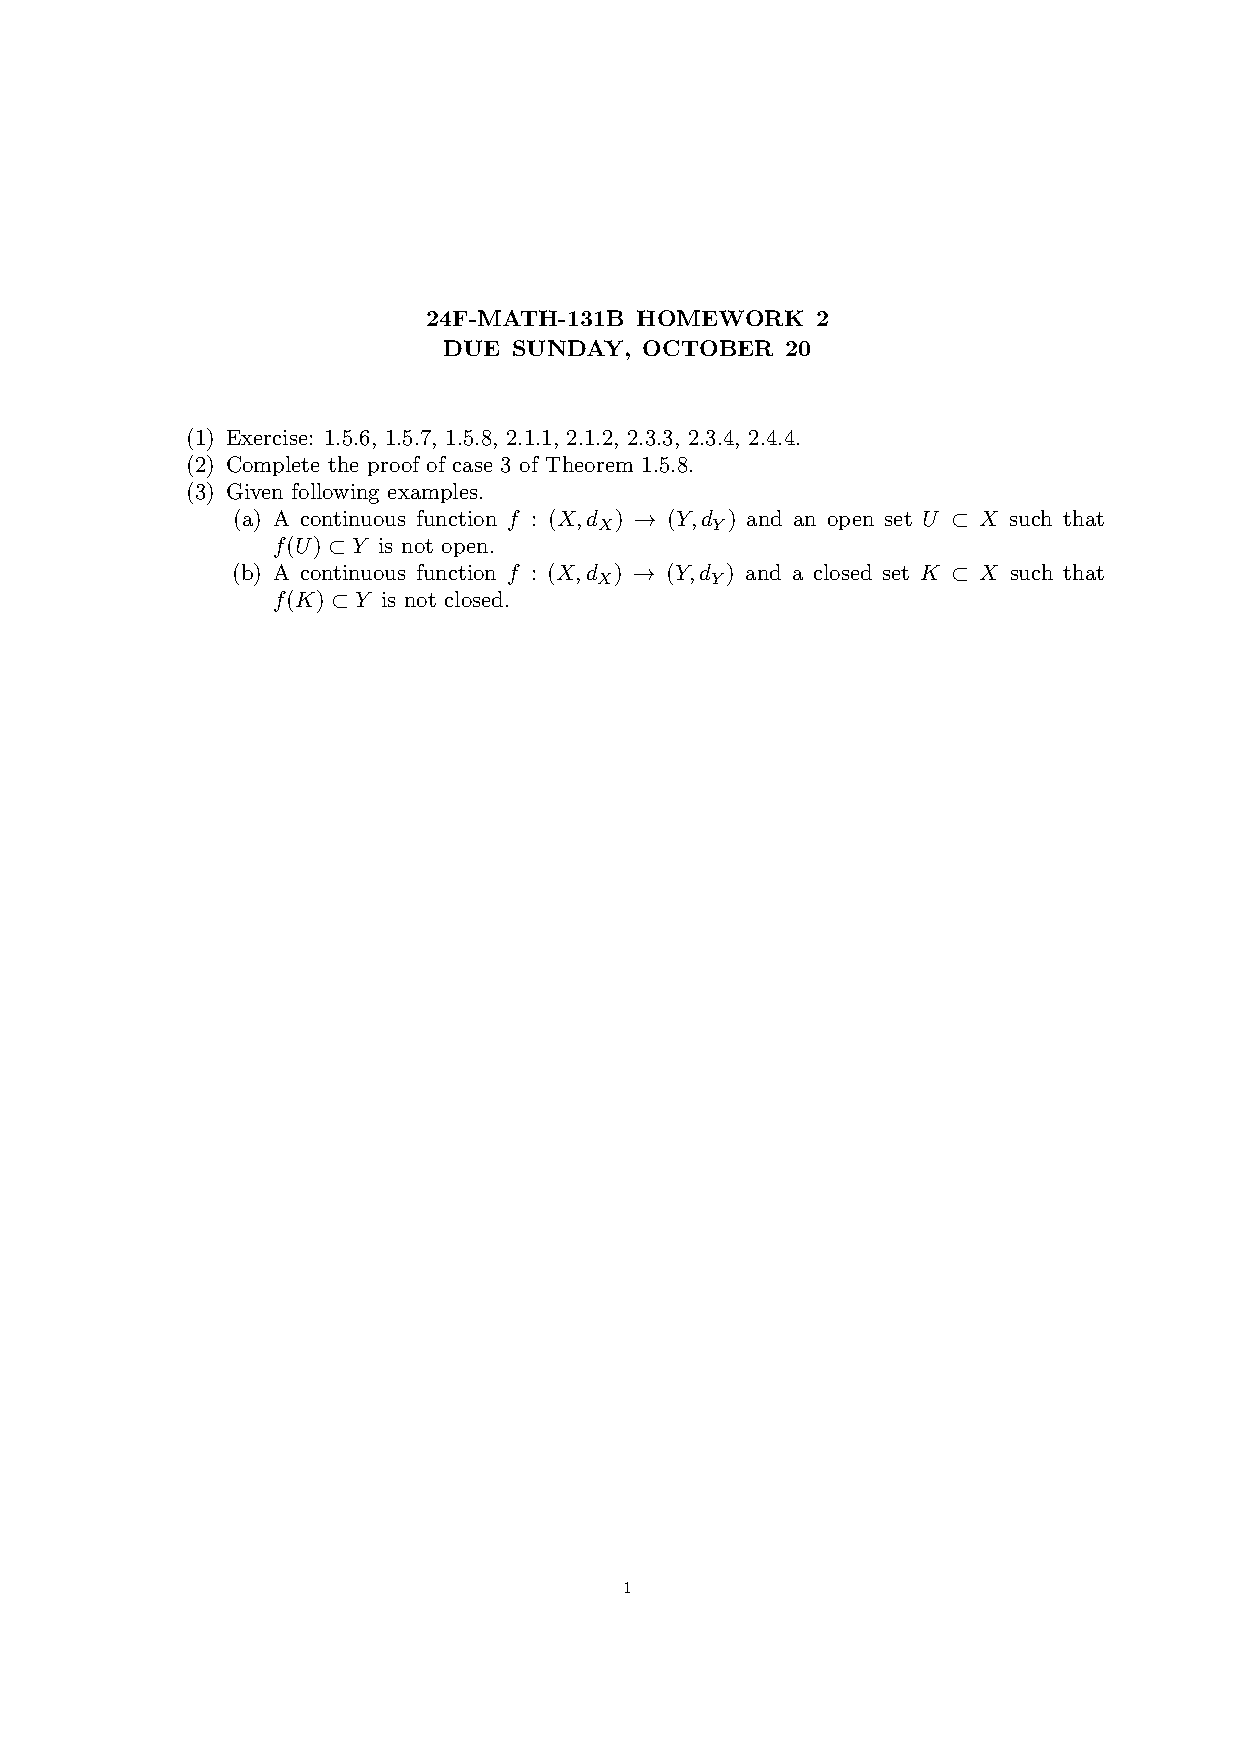
\includepdf[pages=-]{assignment.pdf}

\end{document}
